\documentclass[12pt]{article}
\usepackage{graphicx}
\usepackage[colorlinks,pdfstartview=FitH]{hyperref}

\graphicspath{ {images/} }

\begin{document}

\title{Badger \\ Outlook Add-in}
\date{November 2015}

\begin{titlepage}
    \maketitle
    
    \begin{abstract}
        Badger is a Microsoft Office 2010 Add-in that allows the user to send reminder emails automatically to prompt recipients to respond to requests. Features of the add-in are discussed along with some scenarios to illustrate how Badger operates. A description of the main code (C\#) components is provided.
    \end{abstract}

\end{titlepage}

\tableofcontents{}

\section{Introduction}

The core feature of Badger is to solve the problem of tracking pending email requests and following up. Often people send a carbon copy (CC) or blind carbon copy (BCC) of the email to themselves and these can be organized into a folder of requests pending response, however remembering to review these items and send a follow up request is unreliable at worst and tedious at best. With email communication becoming increasingly process-critical and voluminous, the ability to set-and-forget email follow ups for a variety of time frames is a convenient way to keep your requests moving through the system.

\subsection{Alternatives}

There are standard features of Outlook that provide similar functionality to the auto-follow-up aspects of Badger, but these are annoying and impersonal. Badger makes it look like you yourself are following up and are concerned, ideally making it harder for the person to ignore, psychopaths aside.

\section{Features}

\subsection{Initialization}
\label{sec:initialization}

When the Badger add-in is loaded by Outlook it will create the following three directories:

\begin{itemize}
    \item{Follow-ups/Badger/American}
    \item{Follow-ups/Badger/European}
    \item{Follow-ups/Badger/Honey}
\end{itemize}

These will be used to store the messages Badger is monitoring for follow-up.

\subsection{Basic Operation}

\begin{figure}
    \centering
    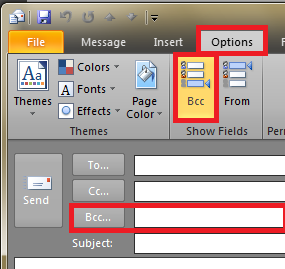
\includegraphics[width=0.5\textwidth]{enable-bcc}
    \caption{You will need to show the BCC field in order to use Badger.}
    \label{fig:enable-bcc}
\end{figure}

Badger will do nothing unless you explicitly identify an email for follow-up. This is done by sending a blind carbon-copy (BCC) of the email to yourself. The BCC option is not available by default, but you can show the BCC field for an email by message by selection the Options tab on the ribbon menu and clicking on BCC in the Show Fields section (see Figure \ref{fig:enable-bcc}).

\begin{figure}
    \centering
    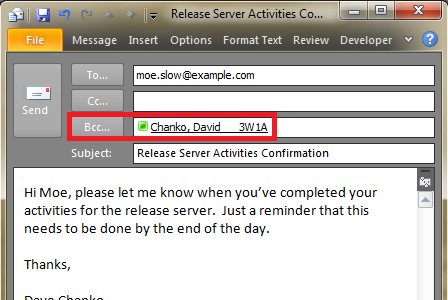
\includegraphics[width=0.5\textwidth]{bcc}
    \caption{BCC yourself to let Badger know you need a follow up.}
    \label{fig:bcc}
\end{figure}

From here you can write your email and add yourself to BCC as shown in Figure \ref{fig:bcc}.

\begin{figure}
    \centering
    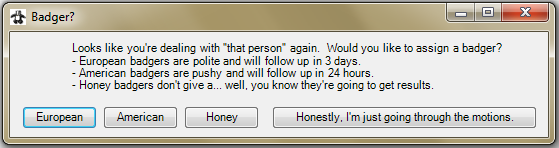
\includegraphics[width=\textwidth]{badger-options}
    \caption{Choose an appropriate follow-up window, if desired.}
    \label{fig:badger-options}
\end{figure}

\begin{table}
    \begin{center}
        \begin{tabular}{ | c | c | }
            \hline
            \textbf{Option} & \textbf{Time Period} \\ \hline
            European & 3 Days \\ \hline
            American & 24 Hours \\ \hline
            Honey & 4 Hours \\ \hline
            Honestly... & No Follow-up \\ \hline
        \end{tabular}
        \caption{Follow-up options and corresponding time periods.}
        \label{tbl:badger-options}
    \end{center}
\end{table}

When you send your email, Badger will recognize that you are BCCing yourself and will prompt you with the window shown in Figure \ref{fig:badger-options}. The options available to you and the respective follow-up period are summarized in Table \ref{tbl:badger-options}.

The forth option of not following up is included in the event you have other follow-up logic/rules setup within Outlook that trigger off of BCCing an email to yourself and you do not want Badger to follow up as well.

If you select one of the first three options Badger will move a copy of your sent email to one of the three folders mentioned in Section \ref{sec:initialization}.  Under normal circumstances you do not need to worry about this.

\begin{figure}
    \centering
    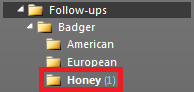
\includegraphics[width=0.5\textwidth]{pending-follow-up}
    \caption{Unread items in the Badger folder identify pending follow-ups.}
    \label{fig:pending-follow-up}
\end{figure}

However, the items moved to the Badger folders will be marked as unread, which provides a nice indicator/confirmation that Badger is monitoring these items for follow-up, as shown in Figure \ref{fig:pending-follow-up}

\subsection{Remove or Undo a Follow-up Request}

Another reason you might care about the folders mentioned in Section \ref{sec:initialization} is when you mistakenly instruct Badger to follow-up on an item, or Badger does not accurately remove an item which has received a follow-up (the logic for this is discussed in Section \ref{sec:handling-replies}). When this happens you can find the message in whichever folder you assigned it to and delete it. This will stop Badger from monitoring and following-up for that item.

\subsection{Handling Replies}
\label{sec:handling-replies}

Badger will mark an item as followed up according to the logic below, which is run on a mail item whenever it is received, or on all mail items in your Inbox folder whenever you open Outlook.

The only way for an item to be considered ``followed-up" is for one of the original ``To" recipients to respond to the message.

Badger examines a mail item's subject and sender fields and attempts to find a mail item in one of its folders where the mail item's subject is found within the subject of the incoming item and the sender of the incoming item is in the list of To addresses of the follow-up item.  If these two conditions are met the follow-up item in the Badger folder will be deleted. The incoming item is left untouched.

\subsubsection{Gaps}

A detailed walk-through of Badger's operation is found in Section \ref{sec:walk-through}, but the basic things to keep in mind are covered here. 

Only incoming mail to your Inbox will be considered by Badger.

If the recipient removes a part of the message subject Badger will not recognize their reply and continue to follow up.

Also, if someone on CC replies to answer your request, Badger will not recognize that as a reply and will continue to follow up.

Lastly, the most seasoned enemies of progress and getting things done will often respond immediately saying ``I'll look at that this afternoon.".  This will count as a response for Badger, so it's up to you to reply saying ``Thanks!", BCCing yourself, and setting up another follow up.

\subsection{Sending Follow-ups}

\subsubsection{Determining a Follow-up is Needed}

While Outlook is open and the Badger add-in is activated, Badger will examine the items in its follow-up folders every five minutes and determine whether or not a follow-up needs to be sent. To do this, Badger uses the time periods identified in Table \ref{tbl:badger-options} and examines the last sent item in the item's conversation to see if the time the most recent item was sent is greater than the follow-up time period.

If an item you marked for follow-up has had replies from those on CC, or from yourself to add more information, Badger will start counting from the latest of these emails when determining whether or not a follow-up will need to be sent.  This means that if you manually follow up on an item in the Badger folders then Badger will wait the specified time period after your manual follow-up before sending its own.

\subsubsection{Creating the Follow-up Email}

\begin{figure}
    \centering
    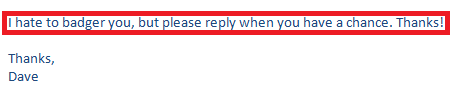
\includegraphics[width=0.75\textwidth]{message}
    \caption{A polite request for a reply will be sent to the original message's ``To" recipients.}
    \label{fig:message}
\end{figure}

The standard follow-up email uses your default reply template and adds the simple message ``Hate to badger you, but please reply when you have a chance. Thanks!". This is sent only to the ``To" recipients of the original email.

If your addressee(s) are particularly stubborn and this is the second time Badger has had to follow up then the first response will be resent, avoiding repeating the same message twice and making you look passive-aggressive. 

\section{Walk-through}
\label{sec:walk-through}

This section provides a sketch of a how all the above features come together and interact in a variety of situations.

Say you send an email to A and B and CC in X and Y.  This is an important matter and time-sensitive so you BCC (figure \ref{fig:bcc}) yourself in order to indicate to Badger you would like to setup a follow-up.  The Badger dialog pops up (figure \ref{fig:badger-options}) and you select ``Honey" for a follow-up after four hours.  

After an hour you realize you forgot to add some important information and reply all adding in the additional details. Badger will track this email and reset the follow-up time to 4 hours after you sent the additional information, a total of 5 hours after the original email was sent.

Another hour passes and X, who was on CC, replies about a parallel task that the full group is interested in. Again, Badger will track this email and reset the follow-up time to 4 hours after it was sent, a total of 6 hours after the original email was sent.

Four more hours pass and no reply is received.  At this point Badger detects that it has been 4 hours since the last email in the chain was sent and sends a polite reminder to only A and B. Still no response before you go home for the day.

When you get into work the next day and open Outlook, Badger will scan your Inbox for any new emails. Not seeing a reply from A or B and it being 4 hours since the last email was sent Badger again follows up to A and B. This time is a little different however, since the last email sent in the chain was another Badger follow-up. Badger detects this and simply resends the previous email without duplicating the polite reminder message.

Finally, after another two hours B replies saying that the task is taken care of, and oh, by the way, that was the politest series of reminders he has ever received in all his years of not paying attention to requests for him to do his job.

\section{Code}

\begin{figure}
    \centering
    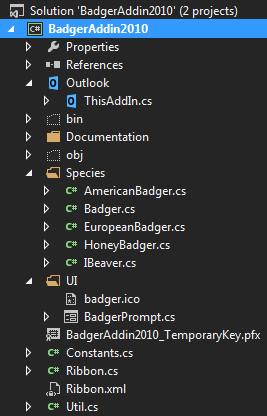
\includegraphics[width=0.5\textwidth]{vs-project}
    \caption{The components of the Badger Visual Studio project.}
    \label{fig:vs-project}
\end{figure}

The code for Badger is very straight-forward and simple, but the project will likely be expanded in the future so starting the documentation now. The project and components are shown in figure \ref{fig:vs-project}.

\subsection{Add-in}

This is where all of Badger's functionality is wired up to Outlook.  Handlers for incoming mail, to detect replies and mark items as followed-up, and sent mail, to detect items that need to be marked for follow-up, are put in place as well as a timer set to trigger every five minutes to scan items pending follow-up to see if any requests for a response should be sent out.

\subsection{UI}

The UI folder contains the WinForms class for the Badger prompt (figure \ref{fig:badger-options}).

\subsection{Badgers}

The Species folder contains the different types of Badgers (see table \ref{tbl:badger-options}) and the root class that contains the logic for handling incoming email and sending follow-ups. The specific Badger classes simply extend and provide values for the folder location and follow-up time period.

\section{Install Badger}

To install Badger download the Badger2010.zip file, extract it, and run the setup.exe file. From here all you need to do is agree to the prompts and restart Outlook.

\section{Remove Badger}

To remove Badger from Outlook go File, Options, Add-Ins, make sure COM Add-ins is selected at the bottom of the screen next to Manage, then click Go\dots .

From the COM Add-Ins window select BadgerAddin2010 and click Remove.

\end{document}
